\documentclass[]{article}
\usepackage{lmodern}
\usepackage{amssymb,amsmath}
\usepackage{ifxetex,ifluatex}
\usepackage{fixltx2e} % provides \textsubscript
\ifnum 0\ifxetex 1\fi\ifluatex 1\fi=0 % if pdftex
  \usepackage[T1]{fontenc}
  \usepackage[utf8]{inputenc}
\else % if luatex or xelatex
  \ifxetex
    \usepackage{mathspec}
  \else
    \usepackage{fontspec}
  \fi
  \defaultfontfeatures{Ligatures=TeX,Scale=MatchLowercase}
  \newcommand{\euro}{€}
    \setmainfont[]{DejaVu Sans}
\fi
% use upquote if available, for straight quotes in verbatim environments
\IfFileExists{upquote.sty}{\usepackage{upquote}}{}
% use microtype if available
\IfFileExists{microtype.sty}{%
\usepackage{microtype}
\UseMicrotypeSet[protrusion]{basicmath} % disable protrusion for tt fonts
}{}
\usepackage[margin=1in]{geometry}
\usepackage{hyperref}
\PassOptionsToPackage{usenames,dvipsnames}{color} % color is loaded by hyperref
\hypersetup{unicode=true,
            pdftitle={1\_Software\_Clusterisation},
            pdfborder={0 0 0},
            breaklinks=true}
\urlstyle{same}  % don't use monospace font for urls
\usepackage{color}
\usepackage{fancyvrb}
\newcommand{\VerbBar}{|}
\newcommand{\VERB}{\Verb[commandchars=\\\{\}]}
\DefineVerbatimEnvironment{Highlighting}{Verbatim}{commandchars=\\\{\}}
% Add ',fontsize=\small' for more characters per line
\usepackage{framed}
\definecolor{shadecolor}{RGB}{248,248,248}
\newenvironment{Shaded}{\begin{snugshade}}{\end{snugshade}}
\newcommand{\KeywordTok}[1]{\textcolor[rgb]{0.13,0.29,0.53}{\textbf{{#1}}}}
\newcommand{\DataTypeTok}[1]{\textcolor[rgb]{0.13,0.29,0.53}{{#1}}}
\newcommand{\DecValTok}[1]{\textcolor[rgb]{0.00,0.00,0.81}{{#1}}}
\newcommand{\BaseNTok}[1]{\textcolor[rgb]{0.00,0.00,0.81}{{#1}}}
\newcommand{\FloatTok}[1]{\textcolor[rgb]{0.00,0.00,0.81}{{#1}}}
\newcommand{\ConstantTok}[1]{\textcolor[rgb]{0.00,0.00,0.00}{{#1}}}
\newcommand{\CharTok}[1]{\textcolor[rgb]{0.31,0.60,0.02}{{#1}}}
\newcommand{\SpecialCharTok}[1]{\textcolor[rgb]{0.00,0.00,0.00}{{#1}}}
\newcommand{\StringTok}[1]{\textcolor[rgb]{0.31,0.60,0.02}{{#1}}}
\newcommand{\VerbatimStringTok}[1]{\textcolor[rgb]{0.31,0.60,0.02}{{#1}}}
\newcommand{\SpecialStringTok}[1]{\textcolor[rgb]{0.31,0.60,0.02}{{#1}}}
\newcommand{\ImportTok}[1]{{#1}}
\newcommand{\CommentTok}[1]{\textcolor[rgb]{0.56,0.35,0.01}{\textit{{#1}}}}
\newcommand{\DocumentationTok}[1]{\textcolor[rgb]{0.56,0.35,0.01}{\textbf{\textit{{#1}}}}}
\newcommand{\AnnotationTok}[1]{\textcolor[rgb]{0.56,0.35,0.01}{\textbf{\textit{{#1}}}}}
\newcommand{\CommentVarTok}[1]{\textcolor[rgb]{0.56,0.35,0.01}{\textbf{\textit{{#1}}}}}
\newcommand{\OtherTok}[1]{\textcolor[rgb]{0.56,0.35,0.01}{{#1}}}
\newcommand{\FunctionTok}[1]{\textcolor[rgb]{0.00,0.00,0.00}{{#1}}}
\newcommand{\VariableTok}[1]{\textcolor[rgb]{0.00,0.00,0.00}{{#1}}}
\newcommand{\ControlFlowTok}[1]{\textcolor[rgb]{0.13,0.29,0.53}{\textbf{{#1}}}}
\newcommand{\OperatorTok}[1]{\textcolor[rgb]{0.81,0.36,0.00}{\textbf{{#1}}}}
\newcommand{\BuiltInTok}[1]{{#1}}
\newcommand{\ExtensionTok}[1]{{#1}}
\newcommand{\PreprocessorTok}[1]{\textcolor[rgb]{0.56,0.35,0.01}{\textit{{#1}}}}
\newcommand{\AttributeTok}[1]{\textcolor[rgb]{0.77,0.63,0.00}{{#1}}}
\newcommand{\RegionMarkerTok}[1]{{#1}}
\newcommand{\InformationTok}[1]{\textcolor[rgb]{0.56,0.35,0.01}{\textbf{\textit{{#1}}}}}
\newcommand{\WarningTok}[1]{\textcolor[rgb]{0.56,0.35,0.01}{\textbf{\textit{{#1}}}}}
\newcommand{\AlertTok}[1]{\textcolor[rgb]{0.94,0.16,0.16}{{#1}}}
\newcommand{\ErrorTok}[1]{\textcolor[rgb]{0.64,0.00,0.00}{\textbf{{#1}}}}
\newcommand{\NormalTok}[1]{{#1}}
\usepackage{graphicx,grffile}
\makeatletter
\def\maxwidth{\ifdim\Gin@nat@width>\linewidth\linewidth\else\Gin@nat@width\fi}
\def\maxheight{\ifdim\Gin@nat@height>\textheight\textheight\else\Gin@nat@height\fi}
\makeatother
% Scale images if necessary, so that they will not overflow the page
% margins by default, and it is still possible to overwrite the defaults
% using explicit options in \includegraphics[width, height, ...]{}
\setkeys{Gin}{width=\maxwidth,height=\maxheight,keepaspectratio}
\setlength{\parindent}{0pt}
\setlength{\parskip}{6pt plus 2pt minus 1pt}
\setlength{\emergencystretch}{3em}  % prevent overfull lines
\providecommand{\tightlist}{%
  \setlength{\itemsep}{0pt}\setlength{\parskip}{0pt}}
\setcounter{secnumdepth}{0}

%%% Use protect on footnotes to avoid problems with footnotes in titles
\let\rmarkdownfootnote\footnote%
\def\footnote{\protect\rmarkdownfootnote}

%%% Change title format to be more compact
\usepackage{titling}

% Create subtitle command for use in maketitle
\newcommand{\subtitle}[1]{
  \posttitle{
    \begin{center}\large#1\end{center}
    }
}

\setlength{\droptitle}{-2em}
  \title{1\_Software\_Clusterisation}
  \pretitle{\vspace{\droptitle}\centering\huge}
  \posttitle{\par}
  \author{}
  \preauthor{}\postauthor{}
  \date{}
  \predate{}\postdate{}


% Redefines (sub)paragraphs to behave more like sections
\ifx\paragraph\undefined\else
\let\oldparagraph\paragraph
\renewcommand{\paragraph}[1]{\oldparagraph{#1}\mbox{}}
\fi
\ifx\subparagraph\undefined\else
\let\oldsubparagraph\subparagraph
\renewcommand{\subparagraph}[1]{\oldsubparagraph{#1}\mbox{}}
\fi

\usepackage{booktabs}
\usepackage{longtable}
\usepackage{array}
\usepackage{multirow}
\usepackage[table]{xcolor}
\usepackage{wrapfig}
\usepackage{float}
\usepackage{colortbl}
\usepackage{pdflscape}
\usepackage{tabu}
\usepackage{threeparttable}
\usepackage{threeparttablex}
\usepackage[normalem]{ulem}
\usepackage{makecell}

\begin{document}
\maketitle

As we discussed, I've filtered the software out of the top 9. As far as
I can judge it might have notable implications further.

Added the binaries such as:\\
- cloudnessBinary\\
- mobileBinary

Relabeled Q4-Q7 such as:\\
- stationaryQuantity\\
- mobileQuantity\\
- cloudnessQuantity

\begin{Shaded}
\begin{Highlighting}[]
\NormalTok{## SOLVED: remake the table with a `q` per `a2`}

\NormalTok{merged =}\StringTok{ }\NormalTok{merged %>%}
\StringTok{  }\KeywordTok{mutate}\NormalTok{(}\DataTypeTok{id =} \DecValTok{1}\NormalTok{:}\KeywordTok{nrow}\NormalTok{(merged)) %>%}\StringTok{ }
\StringTok{  }\KeywordTok{group_by}\NormalTok{(a2, q) %>%}
\StringTok{  }\KeywordTok{mutate}\NormalTok{(}\DataTypeTok{QuantPerDevice =} \KeywordTok{n}\NormalTok{()) %>%}\StringTok{ }
\StringTok{  }\KeywordTok{spread}\NormalTok{(}\DataTypeTok{key =} \NormalTok{q, }\DataTypeTok{value =} \NormalTok{QuantPerDevice, }\DataTypeTok{fill =} \DecValTok{0}\NormalTok{) %>%}\StringTok{ }\KeywordTok{select}\NormalTok{(-id) %>%}
\StringTok{  }\KeywordTok{ungroup}\NormalTok{() %>%}\StringTok{ }\KeywordTok{group_by}\NormalTok{(a2) %>%}\StringTok{ }
\StringTok{  }\KeywordTok{mutate}\NormalTok{(}\DataTypeTok{stationaryQuantity =} \KeywordTok{sum}\NormalTok{(Q4), }\CommentTok{# feature: quantity, software on desktop/laptop}
         \DataTypeTok{mobileQuantitiy =} \KeywordTok{sum}\NormalTok{(Q5 +}\StringTok{ }\NormalTok{Q6), }\CommentTok{# feature: quantity, software on mobile/laptop devices}
         \DataTypeTok{cloudnessQuantity =} \KeywordTok{sum}\NormalTok{(Q7)) %>%}\StringTok{ }\CommentTok{# feature: quantity, software is used on the web (cloud)}
\StringTok{  }\KeywordTok{select}\NormalTok{(-}\KeywordTok{c}\NormalTok{(Q4, Q5,Q6, Q7))}

\CommentTok{# feaure: whether software is principally used on several devices}
\NormalTok{merged$mobileBinary =}\StringTok{ }\KeywordTok{ifelse}\NormalTok{(merged$mobileQuantitiy >}\StringTok{ }\DecValTok{1}\NormalTok{, }\DecValTok{1}\NormalTok{, }\DecValTok{0}\NormalTok{)}
\CommentTok{# feature: whether software is principally possess web version}
\NormalTok{merged$cloudnessBinary  =}\StringTok{ }\KeywordTok{ifelse}\NormalTok{(merged$cloudnessQuantity >}\StringTok{ }\DecValTok{1}\NormalTok{, }\DecValTok{1}\NormalTok{, }\DecValTok{0}\NormalTok{)}
\end{Highlighting}
\end{Shaded}

Adding Q8\_v2\_1:Q16 questions with are ordinal. We treat them close to
numerical in order to make aggregation for the software peaces.

\section{Pre-MDS data preparation,
scaling}\label{pre-mds-data-preparation-scaling}

One of the first plot I showed was MDS without any scaling for
Occupations. Due to the fact that some of the Occupations are simple
over represented it might have (and probably did) affected the
interpretability. Though, current groups of software clustered a bit
better.

\begin{Shaded}
\begin{Highlighting}[]
\NormalTok{## Scaling Before MDS, results are even worse    }
\NormalTok{## UPD: scaling should be accomplished for all of the vars, another fix}

\CommentTok{# pre_dist_multi_final %>% colnames()}

\NormalTok{## scaling only for occupations since they represent absolute frequencies}

\NormalTok{pre_dist_multi_final_no_scaling =}\StringTok{ }\NormalTok{pre_dist_multi_final}
\NormalTok{pre_dist_multi_final[,-}\KeywordTok{c}\NormalTok{(}\DecValTok{1}\NormalTok{,}\DecValTok{2}\NormalTok{)] %<>%}\StringTok{ }\KeywordTok{apply}\NormalTok{(}\DecValTok{2}\NormalTok{, function(X) }\KeywordTok{scale}\NormalTok{(X))}

\NormalTok{## pre_dist_multi_final[,-c(1:3)] %<>% apply(2, function(X) scale(X, center = FALSE))}
\end{Highlighting}
\end{Shaded}

\section{MDS includes all}\label{mds-includes-all}

I tried several distance calculation metrics (`euclidean' `maximum'
`manhattan' `minkowski' `canberra' `binary'). Manhattan is good, though,
canberra - seems to better divide groups. The difference between them is
that canberra is better suited for discrete, while euclidean is the de
facto default for continuous numeric. I wrapped MDS, kmeans and
visualisation into function - you can try different distances, it is the
**\_mds\_with\_Q8**.

\subsection{Figure 1 is the option I suggest to stop on for
now}\label{figure-1-is-the-option-i-suggest-to-stop-on-for-now}

\begin{verbatim}
## [1] "Nothing to exlude"
\end{verbatim}

\begin{figure}[htbp]
\centering
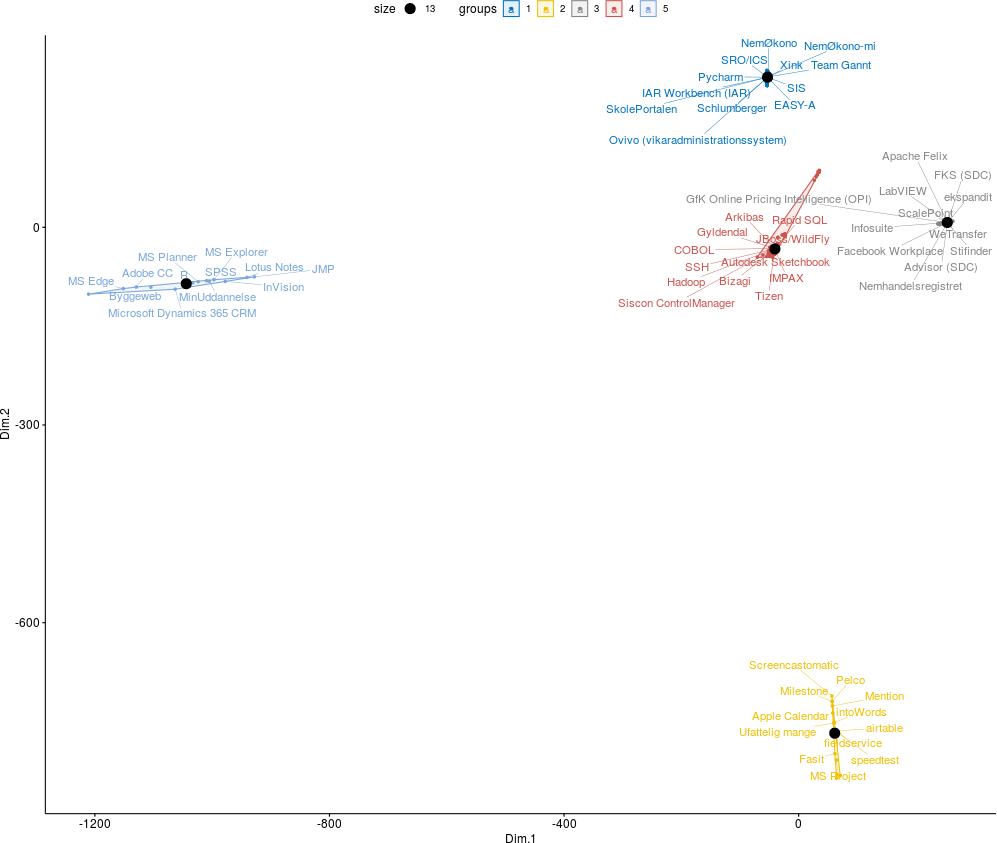
\includegraphics{/home/stlk/projects/appcentriccomp/reports/028_mds_with_Q8_files/figure-latex/unnamed-chunk-12-1.png}
\caption{MDS with all constructs:devices, reprogrammability, occupation}
\end{figure}

\subsection{Different distance used, what I don't like here is that
Apple Contacts and Calendar are in a different
places.}\label{different-distance-used-what-i-dont-like-here-is-that-apple-contacts-and-calendar-are-in-a-different-places.}

\begin{Shaded}
\begin{Highlighting}[]
\NormalTok{p =}\StringTok{ }\KeywordTok{flexible_clustering}\NormalTok{(pre_dist_multi_final, }\DataTypeTok{method =} \StringTok{"manhattan"}\NormalTok{, }\DataTypeTok{clust_n =} \DecValTok{5}\NormalTok{, }\DataTypeTok{labels_col =} \DecValTok{12}\NormalTok{,}
                        \DataTypeTok{column_exclude_start =} \DecValTok{0}\NormalTok{, }\DataTypeTok{column_exclude_end =} \DecValTok{0}\NormalTok{, }\DataTypeTok{seed =} \DecValTok{11}\NormalTok{)$plot}
\end{Highlighting}
\end{Shaded}

\begin{verbatim}
## [1] "Nothing to exlude"
\end{verbatim}

\begin{Shaded}
\begin{Highlighting}[]
\NormalTok{p}
\end{Highlighting}
\end{Shaded}

\begin{figure}[htbp]
\centering
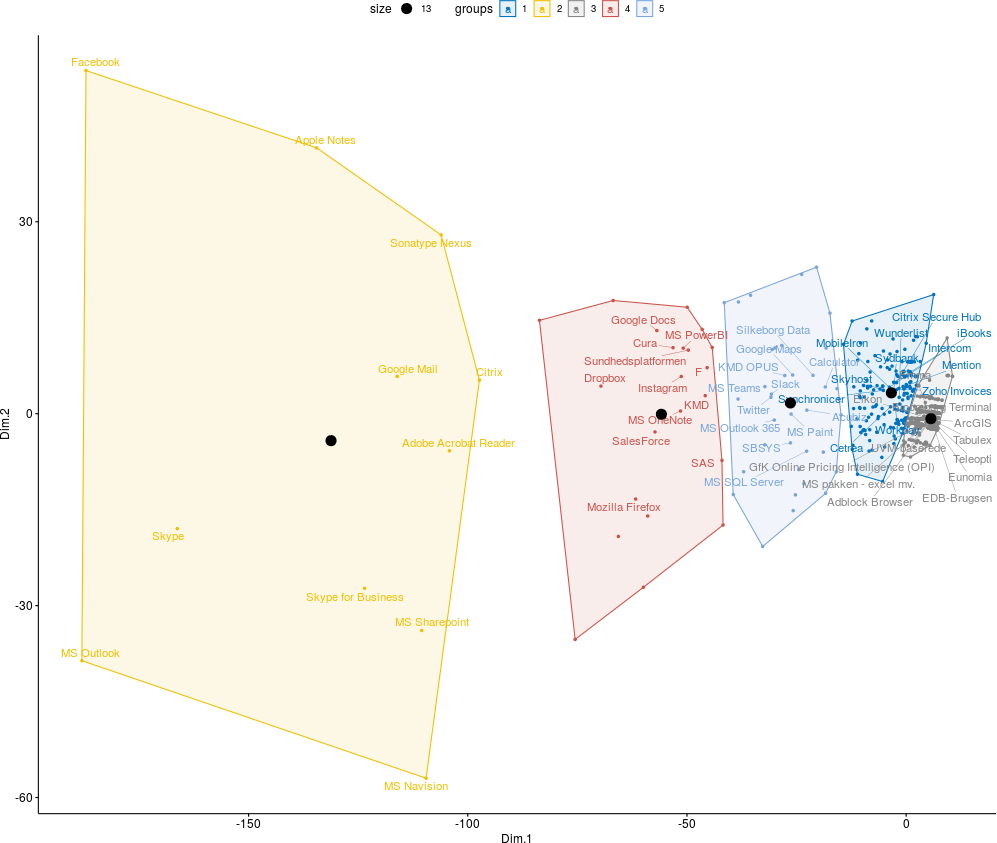
\includegraphics{/home/stlk/projects/appcentriccomp/reports/028_mds_with_Q8_files/figure-latex/unnamed-chunk-13-1.png}
\caption{Mapping Software: Apple Products Appeared in Different
Clusters}
\end{figure}

\section{Others (just take to be aware of
alternatives)}\label{others-just-take-to-be-aware-of-alternatives}

\subsection{MDS: reprogrammability and devices
used}\label{mds-reprogrammability-and-devices-used}

I put it here just to compare with the previous one, I like it much less
than the previous one. Meanwhile, it might be that I just overlooked
something important.

\subsubsection{Canberra distances}\label{canberra-distances}

\begin{Shaded}
\begin{Highlighting}[]
\NormalTok{## pre_dist_multi_final %>% colnames}

\NormalTok{p =}\StringTok{ }\KeywordTok{flexible_clustering}\NormalTok{(pre_dist_multi_final, }\DataTypeTok{method =} \StringTok{"canberra"}\NormalTok{, }\DataTypeTok{clust_n =} \DecValTok{5}\NormalTok{, }\DataTypeTok{labels_col =} \DecValTok{12}\NormalTok{,}
                        \DataTypeTok{column_exclude_start =} \DecValTok{20}\NormalTok{, }\DataTypeTok{column_exclude_end =} \DecValTok{29}\NormalTok{, }\DataTypeTok{additional_exclude =} \KeywordTok{c}\NormalTok{(}\StringTok{"cloudnessBinary"}\NormalTok{,}\StringTok{"mobileBinary"}\NormalTok{),}
                        \DataTypeTok{seed =} \DecValTok{11}\NormalTok{)$plot}

\NormalTok{p}
\end{Highlighting}
\end{Shaded}

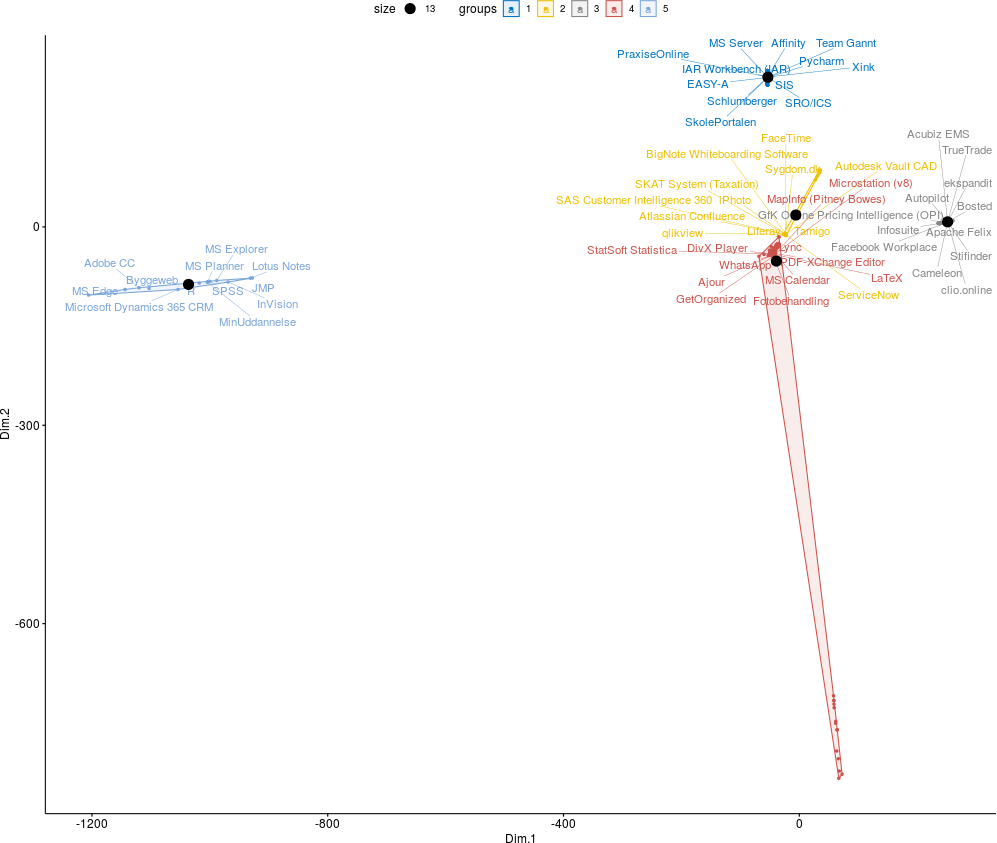
\includegraphics{/home/stlk/projects/appcentriccomp/reports/028_mds_with_Q8_files/figure-latex/unnamed-chunk-14-1.png}

\subsubsection{Euclidean distances}\label{euclidean-distances}

\begin{Shaded}
\begin{Highlighting}[]
\NormalTok{p =}\StringTok{ }\KeywordTok{flexible_clustering}\NormalTok{(pre_dist_multi_final, }\DataTypeTok{method =} \StringTok{"euclidean"}\NormalTok{, }\DataTypeTok{clust_n =} \DecValTok{4}\NormalTok{, }\DataTypeTok{labels_col =} \DecValTok{6}\NormalTok{,}
                        \DataTypeTok{column_exclude_start =} \DecValTok{20}\NormalTok{, }\DataTypeTok{column_exclude_end =} \DecValTok{29}\NormalTok{, }\DataTypeTok{additional_exclude =} \KeywordTok{c}\NormalTok{(}\StringTok{"cloudnessBinary"}\NormalTok{,}\StringTok{"mobileBinary"}\NormalTok{),}
                        \DataTypeTok{seed =} \DecValTok{11}\NormalTok{)$plot}


\NormalTok{p}
\end{Highlighting}
\end{Shaded}

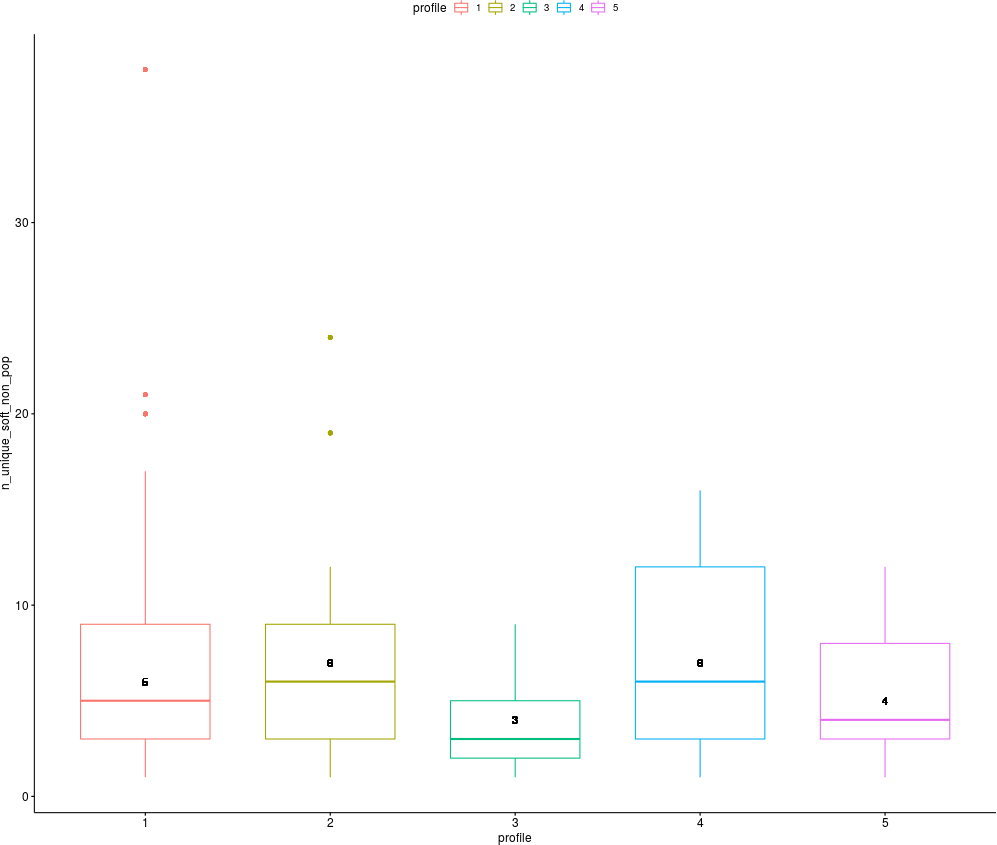
\includegraphics{/home/stlk/projects/appcentriccomp/reports/028_mds_with_Q8_files/figure-latex/unnamed-chunk-15-1.png}

\subsection{MDS: only Occupation}\label{mds-only-occupation}

This one is a bit better.

\begin{Shaded}
\begin{Highlighting}[]
\NormalTok{p =}\StringTok{ }\KeywordTok{flexible_clustering}\NormalTok{(pre_dist_multi_final, }\DataTypeTok{method =} \StringTok{"canberra"}\NormalTok{, }\DataTypeTok{clust_n =} \DecValTok{5}\NormalTok{, }\DataTypeTok{labels_col =} \DecValTok{12}\NormalTok{,}
                        \DataTypeTok{column_exclude_start =} \DecValTok{3}\NormalTok{, }\DataTypeTok{column_exclude_end =} \DecValTok{20}\NormalTok{,}
                        \CommentTok{#additional_exclude = c("cloudnessBinary","mobileBinary"),}
                        \DataTypeTok{seed =} \DecValTok{11}\NormalTok{)$plot}
\end{Highlighting}
\end{Shaded}

\begin{verbatim}
## [1] "Nothing to exlude"
\end{verbatim}

\begin{Shaded}
\begin{Highlighting}[]
\NormalTok{p}
\end{Highlighting}
\end{Shaded}

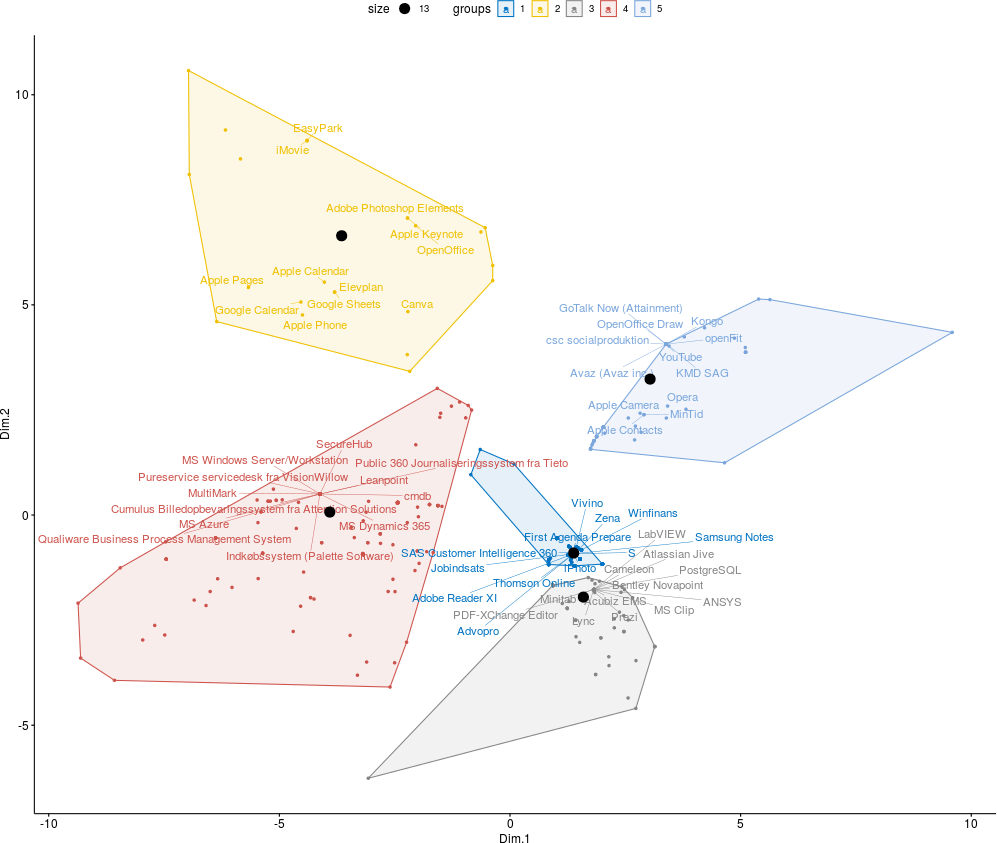
\includegraphics{/home/stlk/projects/appcentriccomp/reports/028_mds_with_Q8_files/figure-latex/unnamed-chunk-16-1.png}

\section{Inspection}\label{inspection}

This table gives an overview of the most typical software items for each
cluster. Raw frequencies are useful to identify goodness of clusters
(some contains much less than others, probably, should think about
decreasing to 4). Scaled might be useful for the description of clusters
using info about professions (health guys use MS Word and few other
software items and that's all). Something similar is given for the
respondents in LPA.

\begin{Shaded}
\begin{Highlighting}[]
\NormalTok{## options(width = 80)}

\NormalTok{inspect =}\StringTok{ }\KeywordTok{flexible_clustering}\NormalTok{(pre_dist_multi_final, }\DataTypeTok{method =} \StringTok{"canberra"}\NormalTok{, }\DataTypeTok{clust_n =} \DecValTok{5}\NormalTok{, }\DataTypeTok{labels_col =} \DecValTok{12}\NormalTok{,}
                              \DataTypeTok{column_exclude_start =} \DecValTok{0}\NormalTok{, }\DataTypeTok{column_exclude_end =} \DecValTok{0}\NormalTok{, }\DataTypeTok{seed =} \DecValTok{11}\NormalTok{)}
\end{Highlighting}
\end{Shaded}

\begin{verbatim}
## [1] "Nothing to exlude"
\end{verbatim}

\begin{Shaded}
\begin{Highlighting}[]
\KeywordTok{inner_join}\NormalTok{(}\KeywordTok{cbind}\NormalTok{(inspect$fit, }\DataTypeTok{labels =} \NormalTok{inspect$labels) %>%}
\StringTok{             }\KeywordTok{select}\NormalTok{(labels, groups),}
           \NormalTok{pre_dist_multi_final_no_scaling, }\DataTypeTok{by =} \KeywordTok{c}\NormalTok{(}\StringTok{"labels"} \NormalTok{=}\StringTok{ "a"}\NormalTok{)) %>%}
\StringTok{  }\KeywordTok{arrange}\NormalTok{(groups) %>%}\StringTok{ }\KeywordTok{select}\NormalTok{(-RecordNo) %>%}
\StringTok{  }\KeywordTok{group_by}\NormalTok{(groups) %>%}\StringTok{ }\KeywordTok{summarise_all}\NormalTok{(}\KeywordTok{funs}\NormalTok{(if(}\KeywordTok{is.numeric}\NormalTok{(.)) }\KeywordTok{sum}\NormalTok{(.) else }\KeywordTok{first}\NormalTok{(.))) %>%}
\StringTok{  }\NormalTok{dplyr::}\KeywordTok{select}\NormalTok{(-labels, -}\KeywordTok{c}\NormalTok{(stationaryQuantity:Q16_agr))  %>%}\StringTok{ }
\StringTok{  }\NormalTok{knitr::}\KeywordTok{kable}\NormalTok{(}\DataTypeTok{digits =} \DecValTok{2}\NormalTok{) %>%}\StringTok{ }\KeywordTok{kable_styling}\NormalTok{(}\DataTypeTok{bootstrap_options =} \StringTok{"striped"}\NormalTok{, }\DataTypeTok{full_width =} \NormalTok{T) }
\end{Highlighting}
\end{Shaded}

\begin{tabu} to \linewidth {>{\raggedright}X>{\raggedleft}X>{\raggedleft}X>{\raggedleft}X>{\raggedleft}X>{\raggedleft}X>{\raggedleft}X>{\raggedleft}X>{\raggedleft}X>{\raggedleft}X>{\raggedleft}X}
\hline
groups & Business and administration & Business, economics, and administration & Chief executives, senior officials, and legislators & General management & Health & Hospitality and retail & ICT & Legal, social, and cultural & Science and engineering & Teaching\\
\hline
1 & 21 & 20 & 6 & 23 & 30 & 2 & 34 & 6 & 12 & 32\\
\hline
2 & 1 & 0 & 0 & 8 & 4 & 0 & 19 & 3 & 9 & 12\\
\hline
3 & 19 & 16 & 2 & 14 & 38 & 2 & 21 & 20 & 24 & 27\\
\hline
4 & 191 & 99 & 59 & 245 & 226 & 22 & 535 & 157 & 246 & 289\\
\hline
5 & 7 & 5 & 0 & 4 & 3 & 1 & 6 & 8 & 15 & 7\\
\hline
\end{tabu}

\begin{Shaded}
\begin{Highlighting}[]
\KeywordTok{inner_join}\NormalTok{(}\KeywordTok{cbind}\NormalTok{(inspect$fit, }\DataTypeTok{labels =} \NormalTok{inspect$labels) %>%}
\StringTok{             }\KeywordTok{select}\NormalTok{(labels, groups),}
           \NormalTok{pre_dist_multi_final, }\DataTypeTok{by =} \KeywordTok{c}\NormalTok{(}\StringTok{"labels"} \NormalTok{=}\StringTok{ "a"}\NormalTok{)) %>%}
\StringTok{  }\KeywordTok{arrange}\NormalTok{(groups) %>%}\StringTok{ }\KeywordTok{select}\NormalTok{(-RecordNo) %>%}
\StringTok{  }\KeywordTok{group_by}\NormalTok{(groups) %>%}\StringTok{ }\KeywordTok{summarise_all}\NormalTok{(}\KeywordTok{funs}\NormalTok{(if(}\KeywordTok{is.numeric}\NormalTok{(.)) }\KeywordTok{mean}\NormalTok{(.) else }\KeywordTok{first}\NormalTok{(.))) %>%}
\StringTok{  }\NormalTok{dplyr::}\KeywordTok{select}\NormalTok{(-labels, -}\KeywordTok{c}\NormalTok{(stationaryQuantity:Q16_agr)) %>%}
\StringTok{  }\NormalTok{## formattable()}
\StringTok{  }\NormalTok{knitr::}\KeywordTok{kable}\NormalTok{(}\DataTypeTok{digits =} \DecValTok{2}\NormalTok{) %>%}\StringTok{ }\KeywordTok{kable_styling}\NormalTok{(}\DataTypeTok{bootstrap_options =} \StringTok{"striped"}\NormalTok{, }\DataTypeTok{full_width =} \NormalTok{T)}
\end{Highlighting}
\end{Shaded}

\begin{tabu} to \linewidth {>{\raggedright}X>{\raggedleft}X>{\raggedleft}X>{\raggedleft}X>{\raggedleft}X>{\raggedleft}X>{\raggedleft}X>{\raggedleft}X>{\raggedleft}X>{\raggedleft}X>{\raggedleft}X}
\hline
groups & Business and administration & Business, economics, and administration & Chief executives, senior officials, and legislators & General management & Health & Hospitality and retail & ICT & Legal, social, and cultural & Science and engineering & Teaching\\
\hline
1 & -0.12 & 0.00 & -0.07 & -0.15 & -0.07 & -0.06 & -0.26 & -0.24 & -0.27 & -0.14\\
\hline
2 & -0.22 & -0.26 & -0.19 & 0.26 & -0.03 & -0.13 & 0.45 & 0.01 & 0.36 & 0.42\\
\hline
3 & -0.17 & -0.10 & -0.16 & -0.24 & -0.07 & -0.08 & -0.34 & -0.13 & -0.21 & -0.21\\
\hline
4 & 0.07 & 0.02 & 0.07 & 0.09 & 0.04 & 0.03 & 0.15 & 0.08 & 0.09 & 0.08\\
\hline
5 & 0.39 & 0.45 & -0.19 & 0.01 & -0.05 & 0.24 & -0.10 & 0.66 & 1.04 & 0.16\\
\hline
\end{tabu}

\begin{Shaded}
\begin{Highlighting}[]
\NormalTok{## inner_join(cbind(inspect$fit, labels = inspect$labels) %>%}
\NormalTok{##              ## filter(labels %in% inspect$selectedLables) %>%}
\NormalTok{##              select(labels, groups),}
\NormalTok{##            pre_dist_multi_final_no_scaling, by = c("labels" = "a")) %>% arrange(groups) %>% select(-RecordNo) %>% }
\NormalTok{##   group_by(groups) %>% summarise_all(funs(if(is.numeric(.)) sum(.) else first(.))) %>% View}



\CommentTok{# cbind(inspect$fit, labels = inspect$labels) %>% filter(labels %in% c("R", "MS Planner"))}
\end{Highlighting}
\end{Shaded}

\section{Understanding Clusters}\label{understanding-clusters}

\subsection{Parallel Coordinates Plot}\label{parallel-coordinates-plot}

This is simple implementation of parallel coordinates. Horizontal lines
here are simply means of clusters. This way, it gives an overview of
what each cluster is about. Since values are scaled, less than 0 - less
than mean, above 0 - above the mean. I included only variables connected
with devices.

\begin{Shaded}
\begin{Highlighting}[]
\NormalTok{parallelCoordsDf =}\StringTok{ }\KeywordTok{inner_join}\NormalTok{(}\KeywordTok{cbind}\NormalTok{(inspect$fit, }\DataTypeTok{labels =} \NormalTok{inspect$labels) %>%}
\StringTok{             }\NormalTok{## filter(labels %in% inspect$selectedLables) %>%}
\StringTok{             }\KeywordTok{select}\NormalTok{(labels, groups),}
             \NormalTok{pre_dist_multi_final_no_scaling, }\DataTypeTok{by =} \KeywordTok{c}\NormalTok{(}\StringTok{"labels"} \NormalTok{=}\StringTok{ "a"}\NormalTok{))}


\NormalTok{parallelCoordsDf$groups %<>%}\StringTok{ }\KeywordTok{as.character}\NormalTok{()}
\NormalTok{parallelCoordsDf$RecordNo %<>%}\StringTok{ }\KeywordTok{as.character}\NormalTok{()}
\NormalTok{parallelCoordsDf %<>%}\StringTok{ }\KeywordTok{group_by}\NormalTok{(groups) %>%}\StringTok{ }\KeywordTok{summarise_all}\NormalTok{(}\KeywordTok{funs}\NormalTok{(if(}\KeywordTok{is.numeric}\NormalTok{(.)) }\KeywordTok{mean}\NormalTok{(.) else }\KeywordTok{first}\NormalTok{(.)))}


\KeywordTok{theme_set}\NormalTok{(}\KeywordTok{theme_classic}\NormalTok{())}

\KeywordTok{ggplot}\NormalTok{(parallelCoordsDf %>%}\StringTok{ }
\StringTok{         }\KeywordTok{mutate}\NormalTok{(}\DataTypeTok{ID =} \DecValTok{1}\NormalTok{:}\KeywordTok{n}\NormalTok{()) %>%}\StringTok{             }
\StringTok{         }\KeywordTok{mutate_if}\NormalTok{(is.numeric, scale) %>%}\StringTok{ }\NormalTok{## FIXME: make global scale before aggregation}
\StringTok{         }\KeywordTok{gather}\NormalTok{(key, value, }\KeywordTok{c}\NormalTok{(}\DecValTok{4}\NormalTok{:}\DecValTok{8}\NormalTok{)),   }
       \KeywordTok{aes}\NormalTok{(key, value, }\DataTypeTok{group=}\NormalTok{groups, }\DataTypeTok{colour =} \NormalTok{groups)) +}\StringTok{ }
\StringTok{  }\KeywordTok{geom_line}\NormalTok{() +}
\StringTok{  }\KeywordTok{geom_vline}\NormalTok{(}\DataTypeTok{xintercept =} \DecValTok{1}\NormalTok{:}\DecValTok{5}\NormalTok{) +}\StringTok{ }
\StringTok{  }\KeywordTok{geom_point}\NormalTok{(}\DataTypeTok{size=}\DecValTok{2}\NormalTok{, }\DataTypeTok{shape=}\DecValTok{21}\NormalTok{, }\DataTypeTok{colour=}\StringTok{"grey50"}\NormalTok{) +}
\StringTok{  }\KeywordTok{scale_fill_manual}\NormalTok{(}\DataTypeTok{values=}\KeywordTok{c}\NormalTok{(}\StringTok{"black"}\NormalTok{,}\StringTok{"white"}\NormalTok{))}
\end{Highlighting}
\end{Shaded}

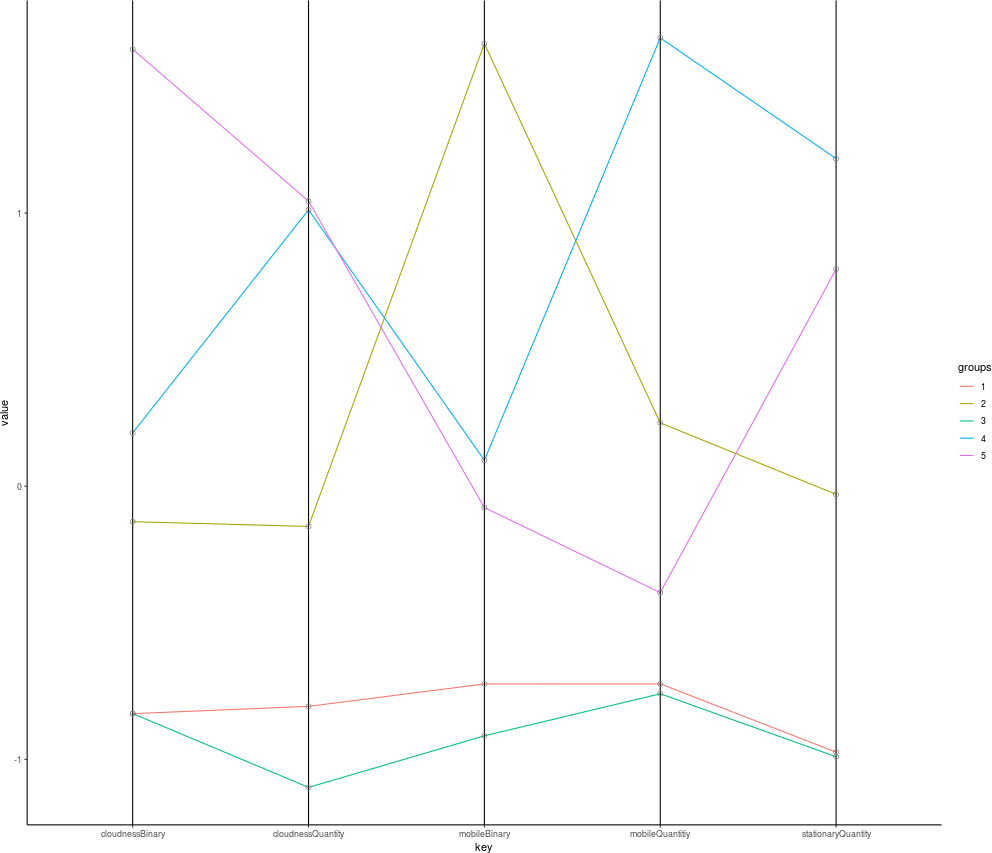
\includegraphics{/home/stlk/projects/appcentriccomp/reports/028_mds_with_Q8_files/figure-latex/unnamed-chunk-19-1.png}

The main point is that mostly Management Systems (CRM systems), Planning
Systems and Software used to Support Collaboration (examples) and
software for software development (tautology** and programming languages
are plotted.

Only 12 software pieces, which are closer to the core of each cluster
are plotted.

\emph{I am describing clusters from Figure 1}

1 cluster:

\begin{itemize}
\tightlist
\item
  low reprogrammability
\item
  nothing specific in terms of device used
\item
  this cluster includes teachers, general management, business, health
  and ICT - very diverse in terms of profession
\item
  from another side, it represents respondents who don't care about
  extensibility of their software toolset
\end{itemize}

Based on the soft used \href{https://www.nemkonto.dk/}{NemOkono},
\href{https://www.iar.com/iar-embedded-workbench/}{IAR Workbench},
\href{https://www.software.slb.com/}{Schlumberger} and
\href{https://www.teamgantt.com/}{Team Gannt}, especially, Pycharm, it
might be about software engineers who do not care about the
extensibility of tools used either about the senior developers/managers,
who rarely programm (Pycharm), but mostly engaged in the planning
activities (Team Gannt - Gannt charts - projects dependencies, seems
like IT approach). Teachers probably use
\href{https://easyiq.dk/skoleportal/}{this}.

Seems like the main logo of this cluster ``This tool is just making the
job need to be done''

2 cluster:

\begin{itemize}
\tightlist
\item
  small cluster in terms of respondents
\item
  managers, ICT, Teachers
\item
  high scores on customasibility of software (less than in 5th cluster,
  more than in 4th)
\item
  prevalence of software used on mobile+tablet type of device
\end{itemize}

Logo: ``Intelligent middle-layer''

Software used: -
\href{https://www.sourcesecurity.com/cctv-software/make.mk-134-ga.html}{Pelco
- CCTV (?)} - system administrators , -
\href{https://schultz.dk/loesninger/schultz-fasit/}{Fasit} -
automatisation job workflow system ? management -
\href{https://www.mv-nordic.com/en/products/intowords/}{intoWords} -
speech-to-text tool, might be used by secretariat -
\href{https://airtable.com/}{airTable} - lightweight and fency web
spreadshit tool -
\href{https://screencast-o-matic.com/}{Screencastomatic} - used for
video capturing - Apple Calendar

3 cluster:

\begin{itemize}
\tightlist
\item
  lowest reprogrammability
\item
  nothing specific in terms of device orientation
\item
  diverse in terms of occupations: business + management + health (+)
  Legal, social and Cultural + Science and Engineering + Teaching
\end{itemize}

Facebook\\
\href{https://wetransfer.com/}{WeTransfer}\\
\href{https://www.infosuite.dk/}{InfoSuite}

Software is rather specific (WeTransfer - file sharing) or has very
broad focus (Facebook).\\
While can't say about the software items, should TODO: check those
users: intuitively, they might use fewer tools than others.

4 cluster:

The majority of the software items are included in this cluster. I
cannot completely understand why mostly items connected with programming
languages and open source are mapped on the plot. \#TODO: use DALEX or
something similar to untangle K-Means clusterisation

\begin{itemize}
\tightlist
\item
  medium repogrammability
\item
  device-specific variables are higher than mean, though, it is the
  biggest cluster, so, don't think it tells a lot
\end{itemize}

COBOL - programming language for business\\
SSH - yeah, well\\
Autodesk Sketchbook - might be proprietary\\
TIZEN - open source\\
Hadoop - should be open sourced\\
\href{Jboss/WildFly}{wildfly} - open source as well

5 cluster:

\begin{itemize}
\tightlist
\item
  small cluster
\item
  mostly stationary and web applications
\item
  highest reprogrammability
\item
  professions: business, no executives, some users are managers, science
  + engineering guys
\end{itemize}

It includes MS Planner, Edge/Explorer,
\href{https://www.rib-software.dk/}{Byggeweb} + R and SPSS + Adobe CC
(outlier, don't like it here). Mostly this cluster has highest score
across reprogrammability. Generally, notable combination of tools with
high reprogrammability with proprietary software without any
customization capabilities. Should inspect it more closely.

Resume: Either we should figure out a better way to map software
considering occupations, either forget about occupation as a measurement
for software.

To try: What I started to doing is Latent Profile Analysis (LPA) (sort
of Dimensionality Reduction specifically for respondents). Since I
didn't completely understand whether it's respondents of software in the
focus (still questionable, right?) I started to describe software using
respondents and vice versa. Instead, maybe, we should consider use
SES-style info in LPA, extract those profiles and try to describe
software based on it (it should solve the issue with sparse occupation
matrix, since, in clustering Occupations doesn't influence the results
that much as expected).

\subsection{Radar Plot}\label{radar-plot}

This is simple implementation of spyder/radar plot. I wasn't a big fan
this kind of plot, but I think I like them now. Also, just additional
line of code in ggplot2.

\begin{Shaded}
\begin{Highlighting}[]
\KeywordTok{ggplot}\NormalTok{(parallelCoordsDf %>%}\StringTok{ }
\StringTok{         }\KeywordTok{mutate}\NormalTok{(}\DataTypeTok{ID =} \DecValTok{1}\NormalTok{:}\KeywordTok{n}\NormalTok{()) %>%}\StringTok{             }
\StringTok{         }\KeywordTok{mutate_if}\NormalTok{(is.numeric, scale) %>%}\StringTok{ }\NormalTok{## FIXME: make global scale before aggregation }
\StringTok{         }\KeywordTok{gather}\NormalTok{(key, value, }\KeywordTok{c}\NormalTok{(}\DecValTok{9}\NormalTok{:}\DecValTok{20}\NormalTok{)),  }
       \KeywordTok{aes}\NormalTok{(key, value, }\DataTypeTok{group=}\NormalTok{groups, }\DataTypeTok{colour =} \NormalTok{groups)) +}\StringTok{ }
\StringTok{  }\KeywordTok{geom_line}\NormalTok{() +}
\StringTok{  }\KeywordTok{geom_vline}\NormalTok{(}\DataTypeTok{xintercept =} \DecValTok{1}\NormalTok{:}\DecValTok{12}\NormalTok{) +}\StringTok{ }
\StringTok{  }\KeywordTok{geom_point}\NormalTok{(}\DataTypeTok{size=}\DecValTok{2}\NormalTok{, }\DataTypeTok{shape=}\DecValTok{21}\NormalTok{, }\DataTypeTok{colour=}\StringTok{"grey50"}\NormalTok{) +}
\StringTok{  }\KeywordTok{scale_fill_manual}\NormalTok{(}\DataTypeTok{values=}\KeywordTok{c}\NormalTok{(}\StringTok{"black"}\NormalTok{,}\StringTok{"white"}\NormalTok{)) +}\StringTok{ }\KeywordTok{coord_polar}\NormalTok{()}
\end{Highlighting}
\end{Shaded}

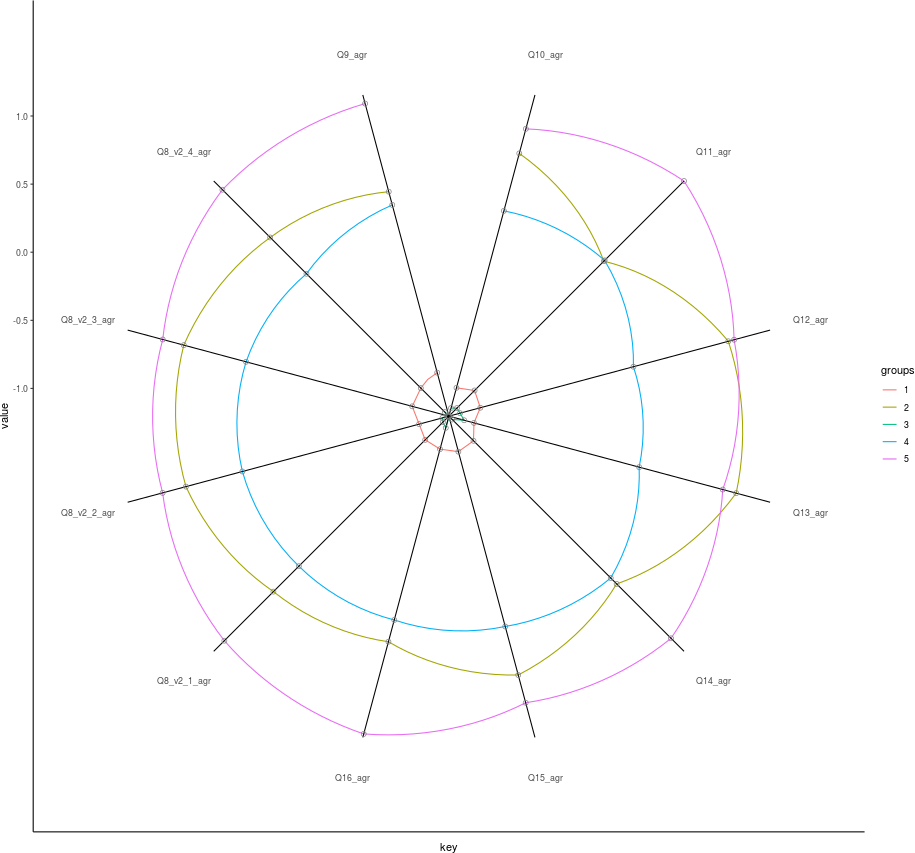
\includegraphics{/home/stlk/projects/appcentriccomp/reports/028_mds_with_Q8_files/figure-latex/unnamed-chunk-20-1.png}

\section{TODO: Use hierarchical clustering
instead}\label{todo-use-hierarchical-clustering-instead}

\end{document}
